%General
\documentclass{article}
\usepackage[utf8]{inputenc}
\usepackage{fullpage}

%Symbols
\usepackage{commath}
\usepackage{amsmath}
\usepackage{amssymb}

%Formatting

%%Automata
\usepackage{tikz}
\usetikzlibrary{arrows,automata}

\usepackage{bussproofs}
\usepackage{hyperref}
\usepackage{amsthm}
\usepackage{alltt}
\newtheorem{theorem}{Theorem}[section]
\newtheorem{definition}[theorem]{Definition}
\newtheorem{example}[theorem]{Example}
\hypersetup{colorlinks=true}
\hypersetup{colorlinks=true}
\usepackage{graphicx}
\graphicspath{ {img/} }
\usepackage{caption}

\title{Title}
\date{\today}
\author{Hjort}

\begin{document}
\maketitle

\section*{DFA}
\subsection*{Basic exercises}

\begin{enumerate}
    \item \textbf{Exercise 2.2.4:} Give DFA's accepting the following languages over the alphabet \{0,1\}:

        All these are validated in the Programs folder in this repository, using Erlang

        \begin{enumerate}
            \item The set of all strings ending in $00$.

                $
                \begin{array}{r | c | c}
                        & 0 & 1 \\ \hline \hline
                    \to q_0 & q_1 & q_0 \\
                        q_1 & q_2 & q_0\\
                        *q_2 & q_2 & q_0
                \end{array}
                $

            \item The set of all strings with three consecutive 0's (not necessarliy at the end)

                $ \begin{array}{r|c|c}
                            & 0 & 1 \\ \hline \hline
                    \to q_0 & q_1 & q_0 \\
                    q_1 & q_2 & q_0 \\
                    q_2 & q_3 & q_0 \\
                    *q_3 & q_3 & q_3
                \end{array}
                $

            \item The set of strings with 001 as a substring

                $ \begin{array}{r|c|c}
                            & 0 & 1 \\ \hline \hline
                    \to q_0 & q_1 & q_0 \\
                    q_1 & q_1 & q_2 \\
                    q_2 & q_1 & q_3 \\
                    *q_3 & q_3 & q_3
                \end{array}
                $

        \end{enumerate}

        % 2
    \item
        A language is a regular language iff it is accepted by some finite automata. We thus construct this automata to prove that this is a regular language.

        $ \begin{array}{r|c|c}
            & 0 & 1 \\ \hline \hline
            \to q_0 & q_1 & q_0 \\
            q_1 & q_1 & q_2 \\
            q_2 & q_3 & q_0 \\
            q_3 & q_4 & q_2 \\
            *q_4 & q_1 & q_2
        \end{array}
        $

        \begin{proof}
            (If part) A string ending in 0100 can be in any state when these last digits are encountered. For every state, we follow the arcs labeled 0,1,0,0 in turn and find we always end in $q_4$, which is an accepting state, so the string is accepted.

            (Only if part) A string has been accepted by the DFA. Since it takes a minimum of 4 transitions to get there, the string must be of at least length 4. We can only reach $q_4$ from $q_3$ following a 0, so the last digit must have been 0. We could only get to $q_3$ from $q_2$, following the arc labeled 0, so the string ends in 00. Every arc into $q_2$ is labeled 1, so the string must end in 100. We can get to $q_2$ only from $q_4$, $q_3$ and $q_1$. All these three states only have arcs labeled 0 going int to them, so the string must end in 0100.
        \end{proof}


    \item

        The state diagram for the DFA accpting words containing $bba$ is seen below.

        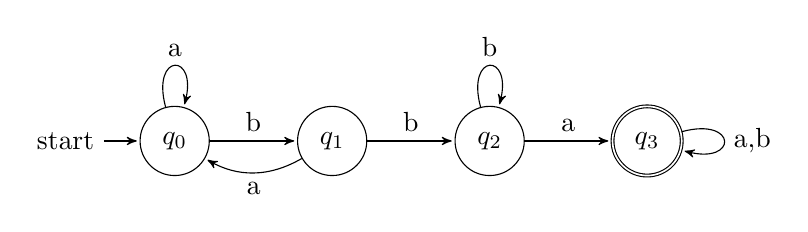
\begin{tikzpicture}[>=stealth',shorten >=1pt,auto,node distance=2cm]
            \node[initial, state]   (q0)    {$q_0$};
            \node[state]            (q1) [right of=q0]    {$q_1$};
            \node[state]            (q2) [right of=q1]    {$q_2$};
            \node[state, accepting] (q3) [right of=q2]    {$q_3$};

            \path[->]
                (q0) edge [loop above]  node {a} (q0)
                     edge   node {b} (q1)
                 (q1) edge  [bend left] node {a} (q0)
                     edge   node {b} (q2)
                (q2) edge   node {a} (q3)
                    edge   [loop above] node {b} (q2)
                (q3) edge  [loop right] node {a,b} (q3);
        \end{tikzpicture}

        The DFA accepting only words without $bba$ as subword must be the words that are not in an accepting state after processing a word with $bba$ as subword, and in an accepting state otherwise. Thus, we simply create an opposite of the DFA above.


        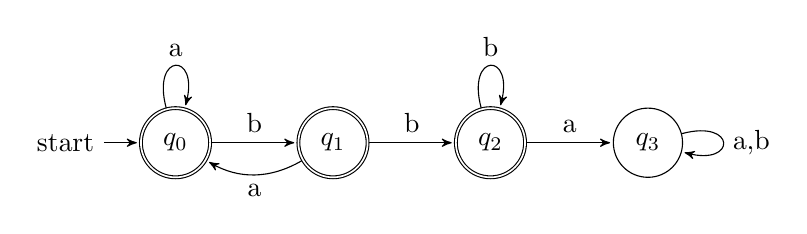
\begin{tikzpicture}[>=stealth',shorten >=1pt,auto,node distance=2cm]
            \node[initial, state, accepting]   (q0)    {$q_0$};
            \node[state, accepting]            (q1) [right of=q0]    {$q_1$};
            \node[state, accepting]            (q2) [right of=q1]    {$q_2$};
            \node[state] (q3) [right of=q2]    {$q_3$};

            \path[->]
                (q0) edge [loop above]  node {a} (q0)
                     edge   node {b} (q1)
                 (q1) edge  [bend left] node {a} (q0)
                     edge   node {b} (q2)
                (q2) edge   node {a} (q3)
                    edge   [loop above] node {b} (q2)
                (q3) edge  [loop right] node {a,b} (q3);
        \end{tikzpicture}
\end{enumerate}


\end{document}
